


\documentclass[a4paper,10pt]{article}
\usepackage{listings,color,epsfig,amsmath,url}
\definecolor{codecolor}{rgb}{0.99,0.97,0.94} % color values Red, Green, Blue
\definecolor{commentcolor}{rgb}{0.1,0.5,0.1} % color values Red, Green, Blue
\definecolor{stringcolor}{rgb}{0.3,0.1,0.1} % color values Red, Green, Blue
\newcommand{\Code}[1]{\texttt{#1} }
\newcommand{\code}[1]{\Code{#1} }
\newcommand{\DB}   {\code{{MOOSDB}}}
\newcommand{\MA}   {\code{{MOOSApp}}}
\newcommand{\Ignore}[1]   {}



% Title Page
\title{Using the Marine Multivehicle Simulator: \code{uMVS} }
\author{Paul Newman}


\begin{document}
\maketitle

\begin{center}

\epsfig{file=images/moose6.eps,width = 0.2\linewidth}
\end{center}
\begin{abstract}
This document will explain how to use the marine multivehicle simulator \code{uMVS}
\end{abstract}



\section{Introduction -- Global Simulation Mode}\label{Sec:SimMode}

There is a mission-file-scope variable \code{simulator}. For
normal operation (i.e. deployment of a real vehicle) this will be
set to be true. However, setting it to \code{false} enters MOOS
into a different mode -- one of simulation.

The idea is that to gain confidence in new code it is a good plan to
be able to do dry runs of all the code that will be expected to
govern the in-life operation of the vehicle. The \code{simulator} flag in
conjunction with the behaviour of the instrument applications can
achieve this.

Setting the \code{simulator} flag to true causes the iProcesses
(instruments) to subscribe to one or more \code{SIM\_*} variables
like \code{SIM\_X},\code{SIM\_Y},\code{SIM\_DEPTH}. These
variables are published by a vehicle simulator (see Section
\ref{sec:uMVS}) and encapsulate the state of a simulated vehicle.
The instruments then simulate their output using these values.

So to summarise: running in simulation mode means all the
instruments, navigation, Helm applications behave as normal,
passing and feeding off the same variables between each other.
However, at the lowest level the instrument classes are not talking
to hardware via their serial ports etc., but are subscribing to data
from a simulated world which they use to generate their
measurements.

For example, iGPS normally talks to a GPS sensor via a serial port
and outputs \code{GPS\_X} etc. In simulation mode it also
subscribes to \code{SIM\_X} and \code{SIM\_Y} which it converts
internally (very simply, it turns out, by using the CMOOSVariable
class) into \code{GPS\_X}.


\begin{figure}[ht]
\centering 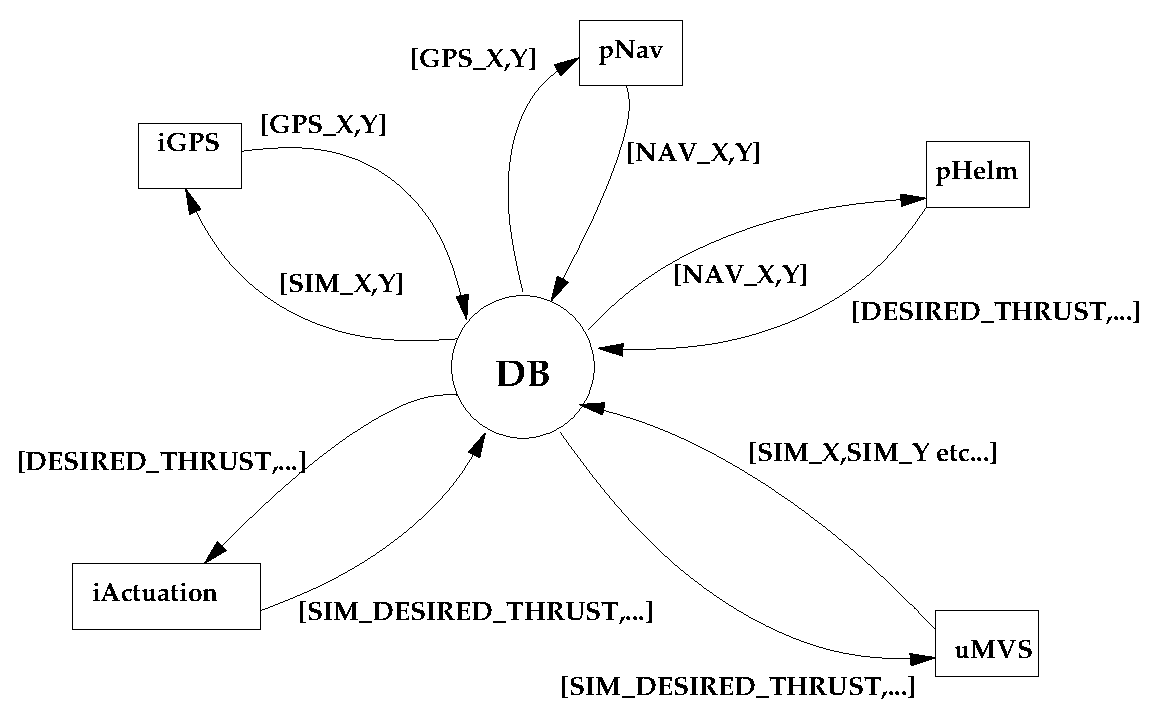
\epsfig{file = images/SimulationMode.eps , width =
0.8\linewidth} \caption{The variable subscription/publication
occurring  in simulation mode }\label{fig:SimulationMode}.
\end{figure}

The final part of the story lies with \code{iActuation} -- when in
simulation this process subscribes as usual to
\code{DESIRED\_RUDDER} etc., but instead of sending bytes via a
serial port to a lump of hardware, it ``re-packages'' the commands
and bounces them back to the \DB as \code{SIM\_DESIRED\_RUDDER}
etc. It is these \code{SIM\_}-prefixed control  variables that are
subscribed to by the simulator and used to control the simulated
vehicle. This scenario is illustrated in Figure
\ref{fig:SimulationMode}. This shows how messages are bounced
around in the simulation mode -- notice the additional \code{SIM\_}
prefixed subscriptions and publications made by \code{iGPS} and
\code{iActuation} respectively.

The details of the simulator are described in Section
\ref{sec:uMVS}.

\section{AUV and Acoustic Simulation  -- \code{uMVS}}\label{sec:uMVS}
\code{uMVS} is a multivehicle AUV simulator. It is capable of
simulating any number of vehicles and acoustic ranging between
them and acoustic transponders. The vehicle simulation
incorporates a full 6D.O.F. vehicle model replete with vehicle
dynamics, center of buoyancy/ center of gravity geometry, and
velocity dependent drag.

The acoustic simulation is also fairly smart. It simulates
acoustic packets propagating as spherical shells through the water
column. When they intersect with acoustic devices (either on
beacons or vehicles) the true time of intersection is calculated
by a refinement process. This design allows the real round trip to
be calculated when the vehicle is undertakes a trajectory that was
not known at the time the initial ``ping'' was launched.

A typical configuration block is given in Figure \ref{fig:uMVSBlock}. The
syntax is simple --- consider the \code{ADD\_AUV} line in Figure
\ref{fig:uMVSBlock}. The initial pose of the vehicle is specified
as an $X,Y,Z,Yaw$ tuple. The AUV can also be named. The
\code{InputPrefix} and \code{OutputPrefix} terms are interesting.
They allow configuration of the names of the variables which are
used to control the actuators of the simulated vehicle and the
names of the variables used to describe the state of the vehicle.
As in reality, each vehicle is controlled by three actuator
settings: rudder, elevator and thrust. On a real vehicle these are
typically carried by the variables
\code{DESIRED\_THRUST}, \code{DESIRED\_ELEVATOR} and
\code{DESIRED\_RUDDER}. Now say a particular simulated vehicle had
\code{InputPrefix = SIM\_}, \code{uMVS} would then subscribe to
\code{SIM\_DESIRED\_THRUST}, \code{SIM\_DESIRED\_ELEVATOR} and
\code{SIM\_DESIRED\_RUDDER} and use these values as the control
parameters for the vehicle. Why might one like to do this? Well,
see Section \ref{Sec:SimMode}. An alternative use of the prefixes
is discussed in Section \ref{Sec:SimMinimal}.

\begin{figure}[h]
\begin{lstlisting}[ ]{}
ProcessConfig = uMVS
{
    //add an AUV, starting at Pose (X,Y,Z,Yaw), called AUV1.
    ADD_AUV=  pose=[4x1]{7,3,55,0},name = AUV1,InputPrefix=SIM_,OutputPrefix=SIM_
    ADD_TRANSPONDER=  name = B1, pose=[3x1]{0,0,0},Rx = CIF, Tx = Ch7,TAT = 0.125

    TideHeight = 60

    //a few variables for the simulator..
    LogFile = SimLog.txt
    InstantLogAcoustics = false

    //what is standard deviation of noise on
    //TOF measurements? 1ms = 1.5 meters
    TOFNoise = 0.00066
}

\end{lstlisting}
\caption{A small configuration block for \code{uMVS} showing a
typical configuration. This would be suitable for use with the
topology shown in Figure \ref{fig:SimulationMode}.
}\label{fig:uMVSBlock}
\end{figure}


\begin{figure}[h]
\begin{lstlisting}[ ]{}
ProcessConfig = uMVS
{
    ....
    ADD_AUV=  pose=[4x1]{7,3,55,0},name = AUV1,InputPrefix=,OutputPrefix=NAV_
    ....
}

\end{lstlisting}
\caption{Configuring the simulator to work for the scenario shown
in Figure \ref{fig:SimpleSim}. }\label{fig:SimpleuMVSBlock}
\end{figure}



\subsection{A More Minimal Simulation}\label{Sec:SimMinimal}

The ability to define the \code{InputPrefix} and
\code{OutputPrefix} terms for \code{uMVS} allows a more minimal
simulation to be constructed without using the global
\code{simulator} flag discussed in Section \ref{Sec:SimMode}.
In fact, one can eschew the need to use the instruments and
\code{iActuation} altogether. Why would anyone want to do this?
Well, the ``simulation mode'' of Section \ref{Sec:SimMode} is
invaluable for gaining overall system/architecture confidence;
however it can be inconvenient at times. For example, if working on
the Helm or action planning process it may be inconvenient  to
have to launch the instrument processes and the Navigator
frequently during development. Figure \ref{fig:SimpleSim} shows an
alternative use of the simulator for exactly this case.  The
important configuration line (compared to Figure \ref{fig:uMVSBlock}) is
shown in Figure \ref{fig:SimpleuMVSBlock}. Note how the simulator
is told to publish \code{NAV\_*} data and subscribe to
\code{DESIRED\_THRUST}, \code{DESIRED\_ELEVATOR}, \code{DESIRED\_RUDDER}
by having an empty input prefix and \code{NAV\_} as an output
prefix. A typical topology using this set up is shown in Figure
\ref{fig:SimpleSim}.

\begin{figure}[ht]
\centering 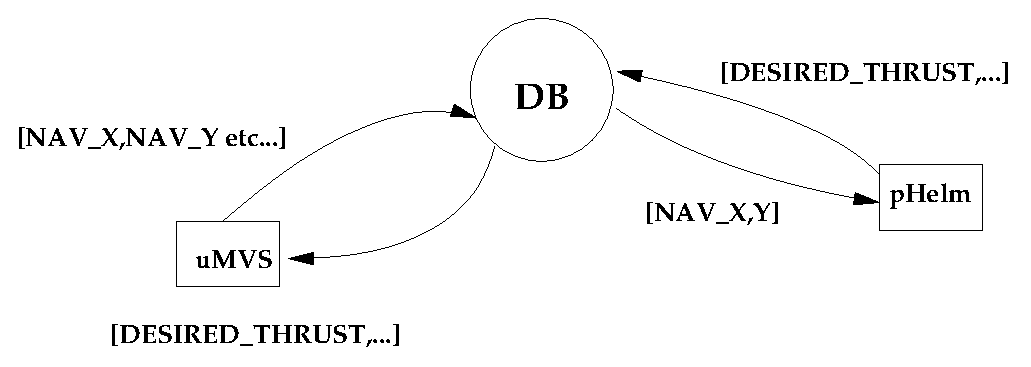
\epsfig{file = images/SimulationMode2.eps , width =
0.8\linewidth} \caption{A minimal simulation configuration, for
example Helm development. Here \code{uMVS} publishes vehicle
state as \code{NAV\_*} data and controls the internal simulated
vehicle by direct subscription to the standard Helm outputs.
}\label{fig:SimpleSim}
\end{figure}

\subsection{Logging}

\code{uMVS} can be configured (via the  \code{ LogFile} parameter)
to write a log file of the simulation. This is a self
documenting file that records vehicle state and acoustic ranges
for perusal outside of the MOOS environment.


\section{Multivehicle Simulation Scenarios}

So far we have considered the case of simulating a single vehicle
community (one community per vehicle). In the case that there is one
mission file for the community, the simulator variable is set to
true and all processes run as though this were a real deployment,
but behind the scenes the simulator is talking to the instruments
to fake reality. This was described in Section \ref{Sec:SimMode}.

However, what if it was desired to simulate (i.e. prepare for) and
experiment with multiple interacting vehicles (i.e. lots of
communities), how would this work? Several options are available to
the user here and they all involve the use of \code{pMOOSBridge},
which is described in the document on MOOSBridge.

One option is to run one simulator for each vehicle (each
simulator only running one vehicle) and use \code{pMOOSBridge} to
bridge whatever variables that need to be shared between
communities (it will most likely need to rename the variables
as well). For example, consider Figure \ref{fig:MultiSim1}. Here a
possible two-vehicle simulation topology is shown. It is created
simply by linking two communities, each with their own private
\code{uMVS} (here each in full simulation mode as described in
Section \ref{Sec:SimMode} but they could of course be in a reduced
form as described in Section \ref{Sec:SimMinimal}) with an
instance of \code{pMOOSBridge} as described in the MOOSBridge document.

\begin{figure}[ht]
\centering 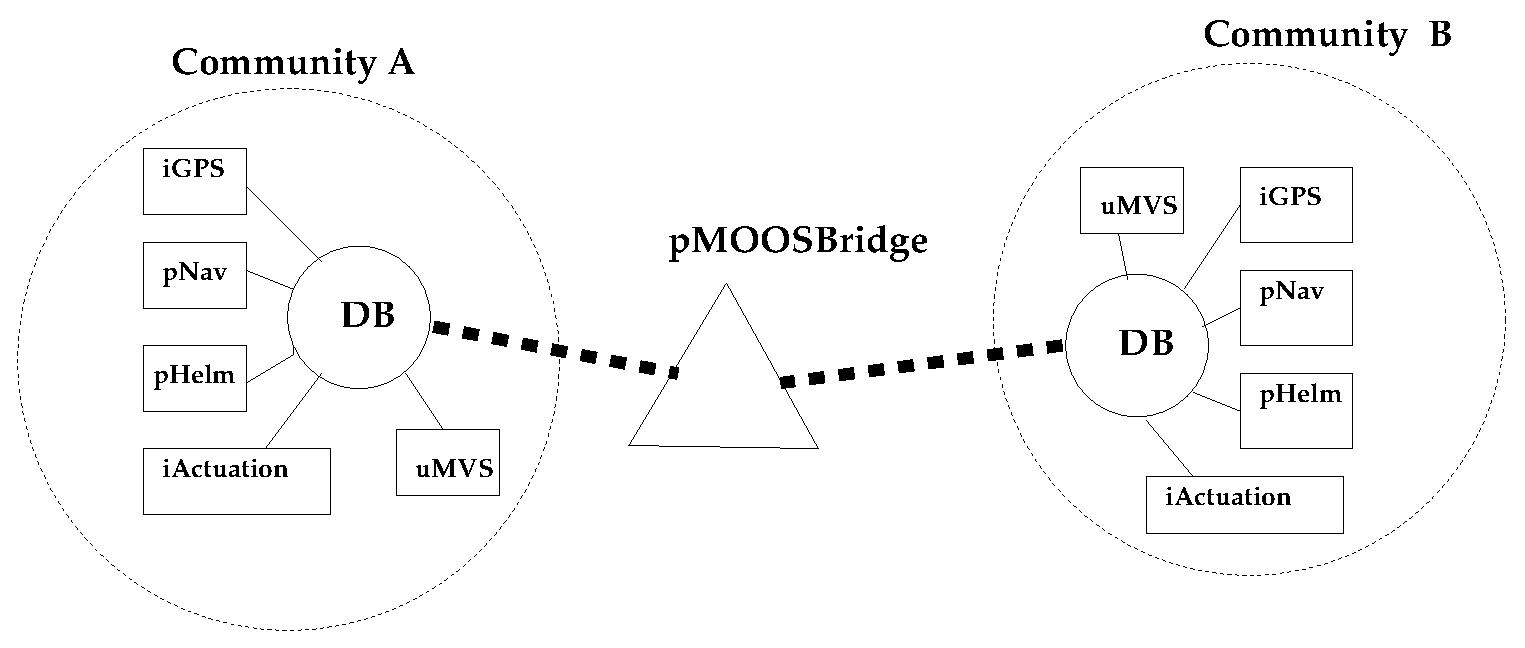
\epsfig{file = images/SimBridge0.eps , width = 0.8\linewidth}
\caption{A possible two-vehicle simulation created simply by
linking two communities each with a private \code{uMVS}(here each
in full simulation mode as described in Section \ref{Sec:SimMode}
but they could of course be in a reduced form as described in
Section \ref{Sec:SimMinimal}) with an instance of
\code{pMOOSBridge}.
 }\label{fig:MultiSim1}
\end{figure}


An alternative  approach would be to use the multivehicle
simulation capabilities of \code{uMVS} and adopt a topology
similar to Figure \ref{fig:MultiSim2}. Here each community has its
vehicle simulated in a common instance of \code{uMVS} which would
allow acoustic ranging between vehicles. Figure
\ref{fig:2AUVBlock} shows the possible configuration block for
\code{uMVS} in this scenario. Each vehicle community in Figure
\ref{fig:MultiSim2} runs its own instance of \code{pMOOSBridge} to
do the relevant data renaming between the ``simulating community''
and the rest of its own community. For example, with reference to
the configuration snippet in Figure \ref{fig:2AUVBlock} and the
topology of Figure \ref{fig:MultiSim2}, the bridge in ``Community
A'' would have to import \code{AUV\_A\_X} from the simulation
community and map it to \code{SIM\_X} while also exporting
\code{SIM\_DESIRED\_THRUST} as \code{AUV\_A\_DESIRED\_THRUST}
\footnote{And similarly for other relevant variables.}.

\begin{figure}[ht]
\centering 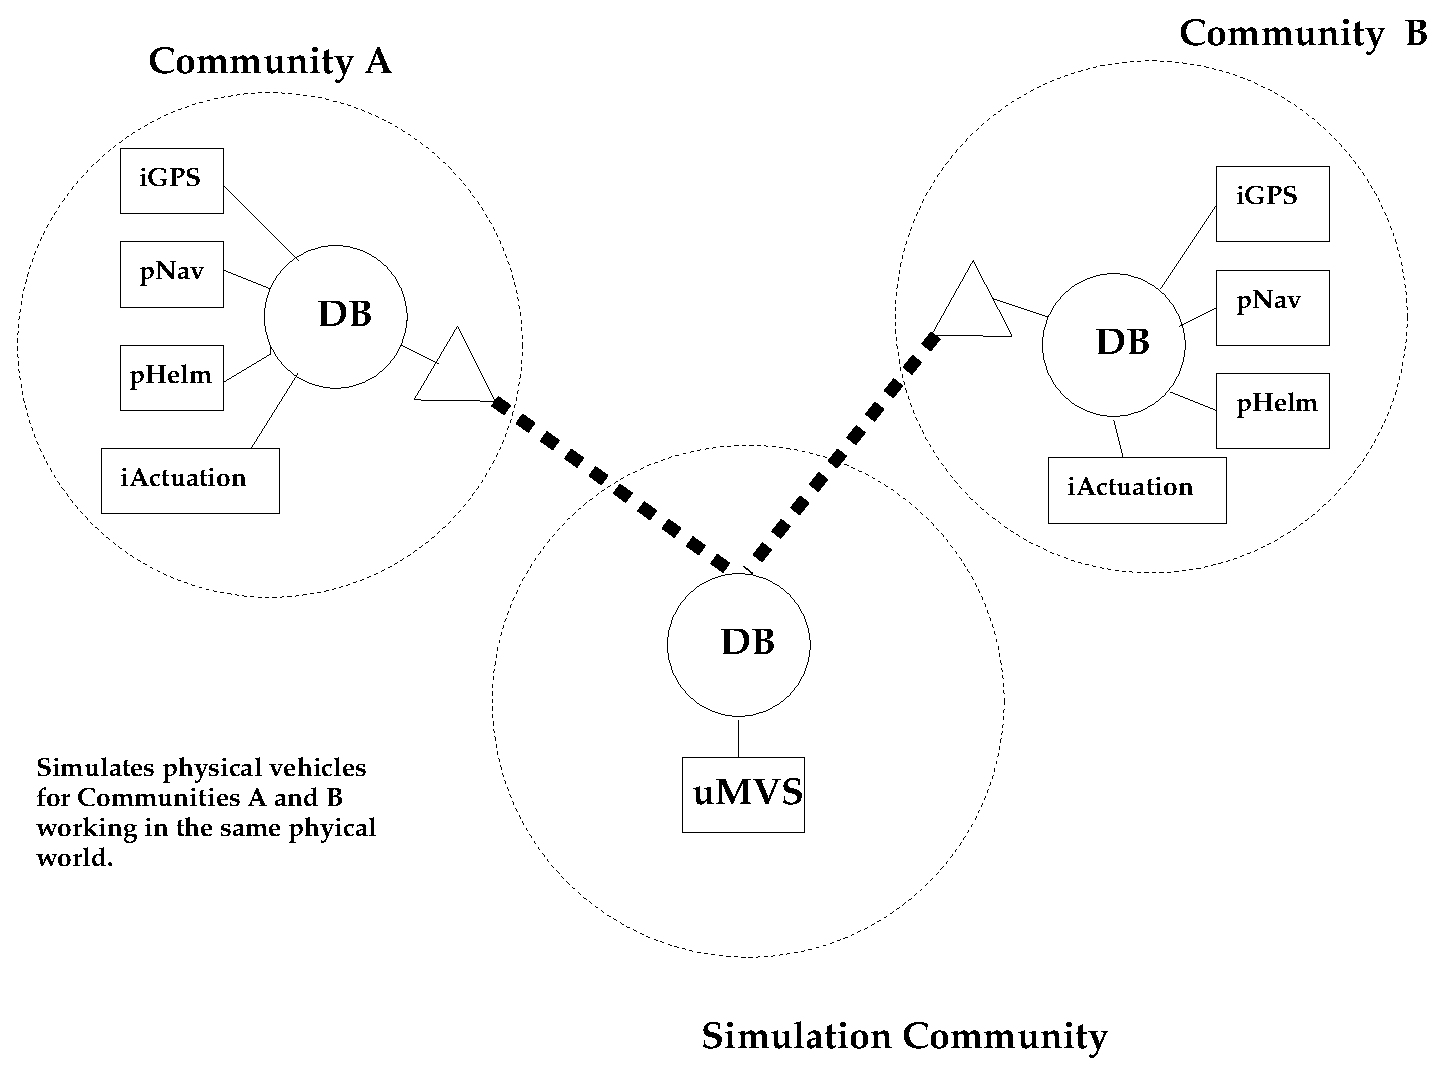
\epsfig{file = images/SimBridge.eps , width = 0.8\linewidth}
\caption{A possible two-vehicle simulation created simply by
linking two communities to a single ``simulation community'' via
private instances of \code{pMOOSBridge}. There is only one
\code{uMVS} running.
 }\label{fig:MultiSim2}
\end{figure}

\begin{figure}[ht]
\begin{lstlisting}[ ]{}
ProcessConfig = uMVS {
    ....
    ADD_AUV=  pose=[4x1]{7,3,55,0},name = VehA,InputPrefix=AUV_A_,OutputPrefix=AUV_A_
    ADD_AUV=  pose=[4x1]{7,3,55,0},name = VehB,InputPrefix=AUV_A_,OutputPrefix=AUV_B_
    ....
}
\end{lstlisting}
\caption{Configuring the simulator to work for the scenario shown
in Figure \ref{fig:MultiSim2} with two vehicles. Note the values
of the input and output prefixes and the message renaming role
each \code{pMOOSBridge} has in Figure \ref{fig:MultiSim2} because
of them }.\label{fig:2AUVBlock}
\end{figure}



\begin{figure}[ht]
\centering 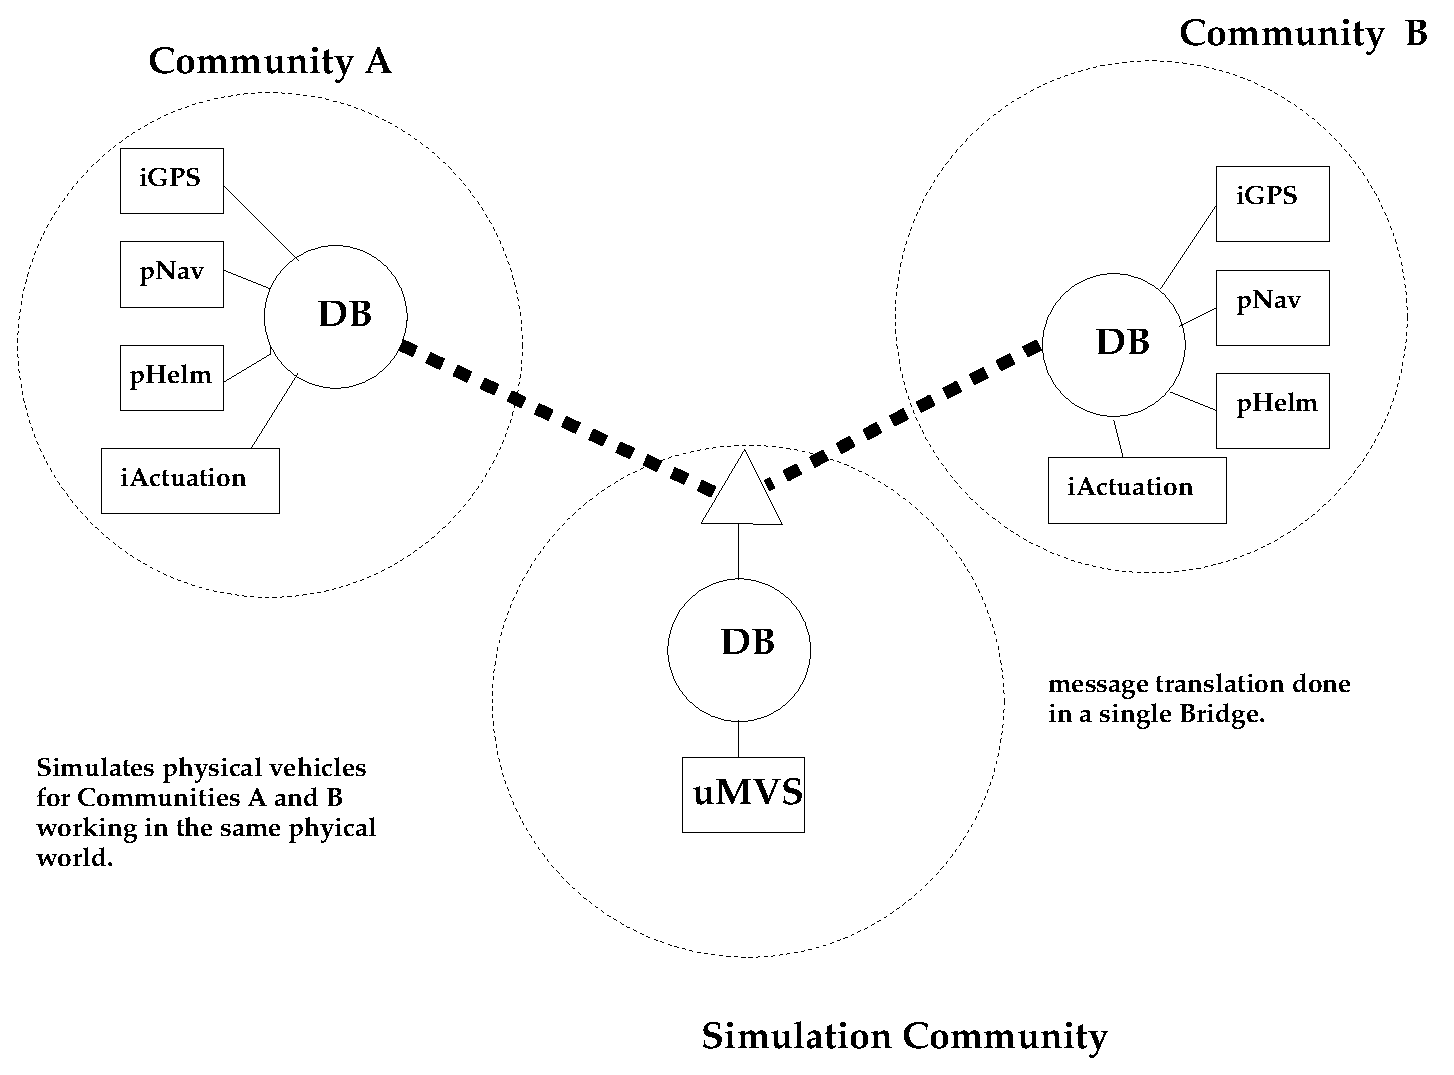
\epsfig{file = images/SimBridge2.eps , width = 0.8\linewidth}
\caption{A possible two-vehicle simulation created simply by
linking two communities to a single ``simulation community'' via a
{\emph{single}} instance of \code{pMOOSBridge}. Again, there is
only one \code{uMVS} running.
 }\label{fig:MultiSim3}
 \end{figure}

\begin{figure}[ht]
\centering 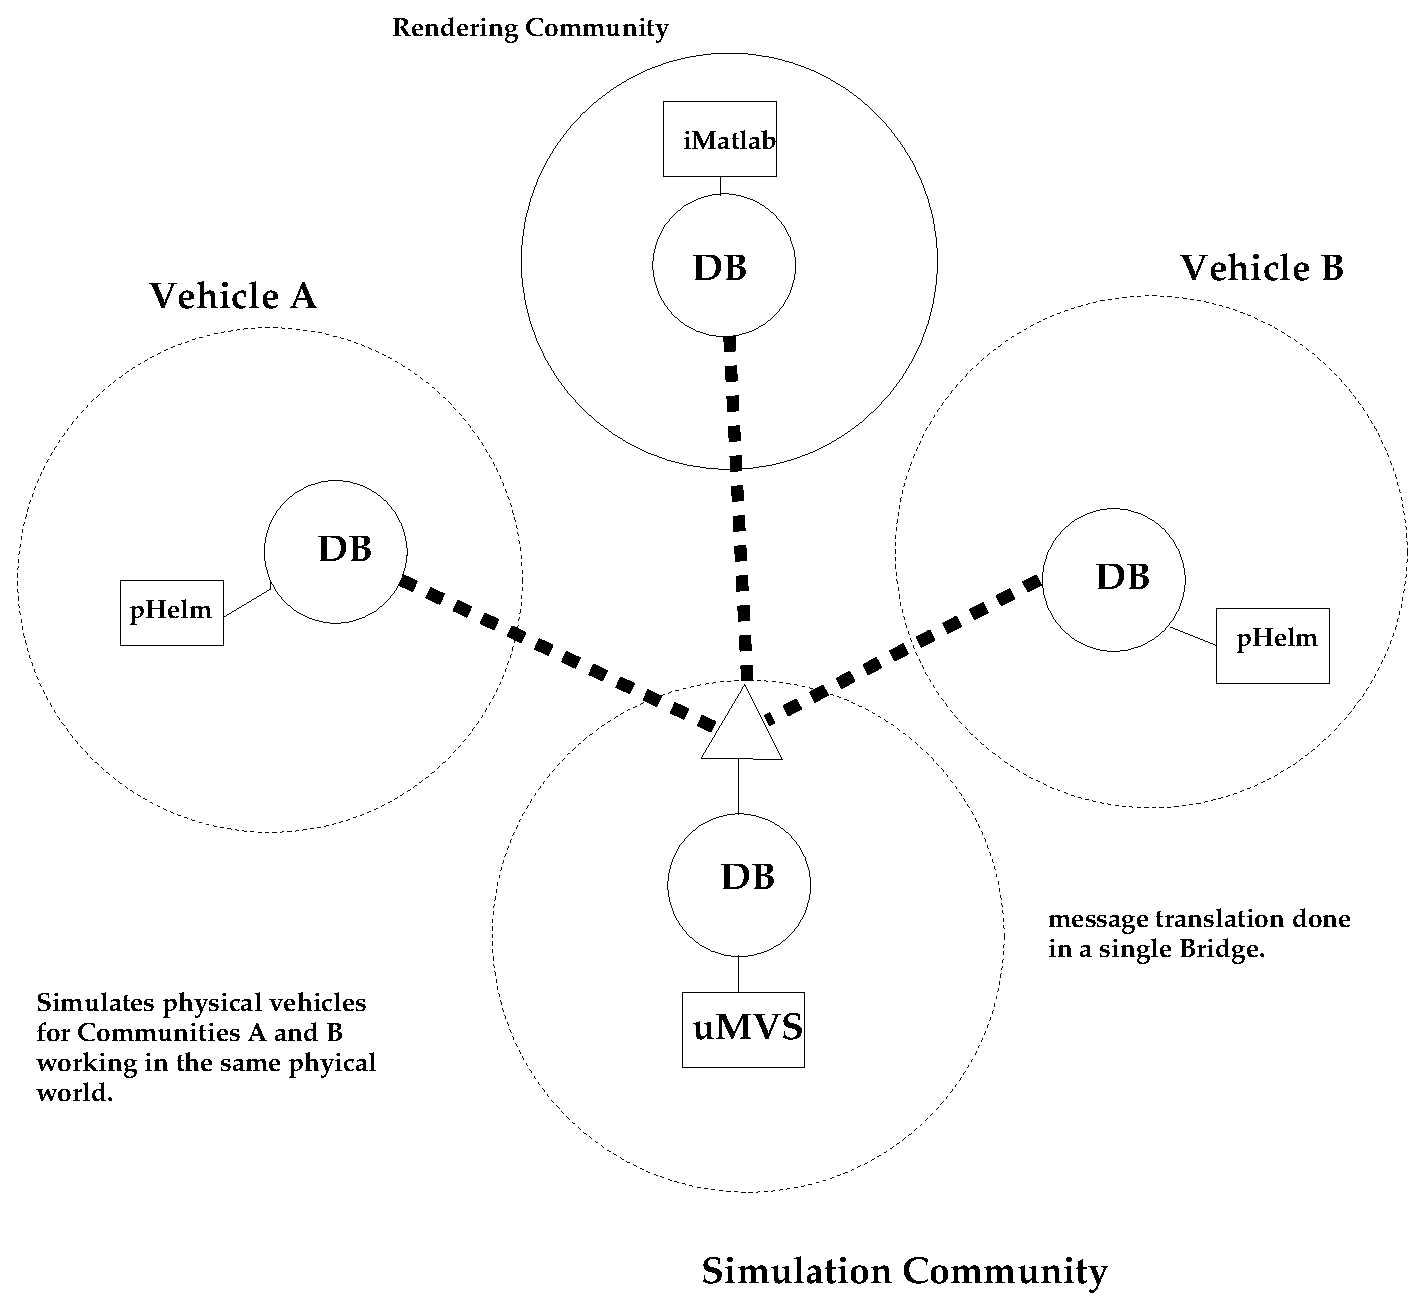
\epsfig{file = images/SimBridge3.eps , width = 0.8\linewidth}
\caption{Similar to Figure \ref{fig:MultiSim3}, where a two-vehicle
simulation is created simply by linking two communities to a
single ``simulation community'' via a {\emph{single}} instance of
\code{pMOOSBridge}. Again, there is only one \code{uMVS} running.
The difference between this topology and that shown in Figure
\ref{fig:MultiSim3} is the individual vehicle communities are
{\emph{not}} running in simulation mode (described in Section
\ref{Sec:SimMode}). Instead, in this case, the single instance of
\code{pMOOSBridge} is renaming and routing data such that the need
for instruments and the navigator is avoided.
 }\label{fig:MultiSim4}
 \end{figure}
Finally, another two alternatives are presented in Figures
\ref{fig:MultiSim3} and \ref{fig:MultiSim4}. Here a single bridge
is used to do all the required data routing and name mapping for
both communities. In Figure \ref{fig:MultiSim4}, a visualisation
community has been added, which uses the \code{iMatlab} interface
to render the simulation in a ``fancy fashion''. Note that in this
case a minimal simulation is being run and so the Bridge will be
mapping, for example, \code{AUV\_A\_SIM\_X} on the simulation
community to \code{NAV\_X} on community \code{A} as well as
\code{AUV\_B\_SIM\_X} to \code{NAV\_X} on community \code{B}.

\subsection{Inter-vehicle Ranging}
The ``ADD\_AUV'' string can also specify how the vehicle acoustic system
responds to acoustic interrogation. By adding something of the form
``{\it{ResponderChannel = Ch3,TAT = 0.125}}'' to the ``ADD\_AUV'' string,
the vehicles will act like acoustic beacons (only they move) and respond to ``CIF'' pulses
from other vehicle transceivers on the channel specified with the declared turnaround time.
If the ``ResponderChannel'' is not specified, it will be assumed that inter-vehicle ranging
is not wanted and the vehicle's acoustic responders will be turned off.

\end{document}
